%===================================== CHAP 3 =================================
\chapter{State of the Art Survey}
\label{ch:related-work}
This chapter gives an overview of some of the research related to this master thesis.
This master thesis is based on the work by Rudihagen \cite{master-thesis} and my project report \cite{project-report}.
The first section introduces the previous work.

\section{Previous Work}
\label{sec:previous-work}
This master thesis is a continuation of the work done by Rudihagen \cite{master-thesis} and my project report \cite{project-report}.
Rudihagen looked at how search engines could return more relevant search results,
but at the same time deliver the results fast enough to be used in live searches.
He looked at how Google Play\footnote{\url{https://play.google.com}} ranked search results.
Google Play is the official app store for Android phones.
He found that Google Play's search results ranked the most popular apps highest.
Ranking the most popular apps highest will result in relevant results in many cases,
but it will also make less popular apps almost dissapear.
By utilizing the techniques Kullback-Leibler divergence and Bayesian classification,
he was able to return more relevant search results.
However, the latency in his implementations ranged from 80 ms to 600 ms.
This means that most of the time the search implementation is too slow to be used in a live search.
The requirement for interactive applications are 100 ms.

The sequence diagram from Rudihagen's query expansion implementation can be seen in figure \ref{fig:sequence-diagram-rudihagen}.
The sequence diagram shows that the query expansion have two round trips from the web server to the search engine,
and two round trips from web server to the database.
Which is a total of four round trips from the web server to collect the data needed for the query expansion algorithm.
According to Rudihagen the measured latency were between 150 ms - 600 ms, and 238 ms on average.

To improve Rudihagen's implementation the assumption were to decrease the number of round trips.
This assumption is based on the results of Rudihagen's other implementations.
His other two implementations had one and two round trips,
with average latencies of 92 and 108 respectively.
This suggest that the number of round trips have a significant impact on the measured latency.

\begin{figure}[h!]
  \centering 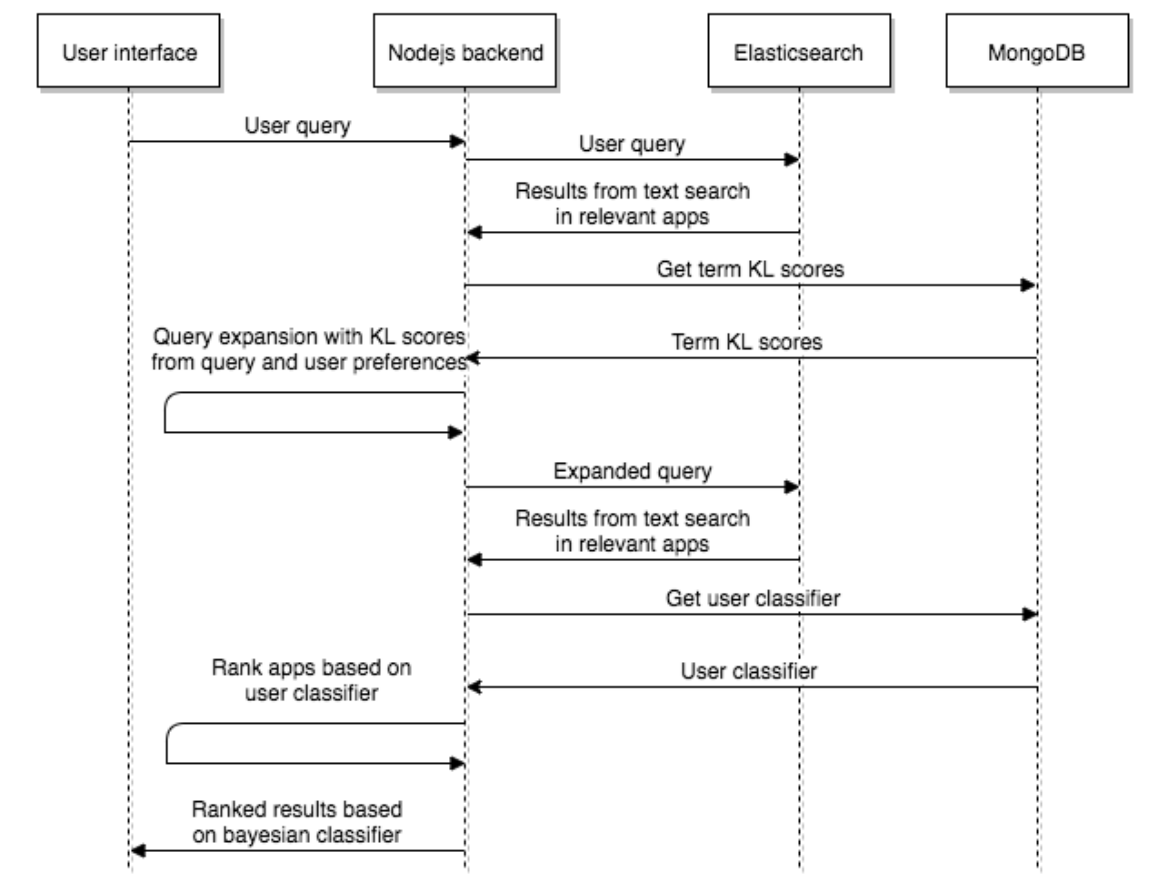
\includegraphics[width=1\linewidth]{img/sequence-diagram-rudihagen.png}
  \caption{Sequence diagram from Rudihagen's implementation of query expansion. Figure taken from \cite{master-thesis}.}
  \label{fig:sequence-diagram-rudihagen}
\end{figure}

Based on the experience from Rudihagen's master thesis,
the project report \cite{project-report} implemented query expansion with less round trips.
The project report describes an implementation which were able to achieve a total of two round trips between the web server and the search engine.
The measured response times was well within the limit of 100 ms.
An important remark is that all the tests described were done on a locally.
If the test were conducted with the server placed at a hosting provider,
the response times would most likely have been higher.

The project report had two different implementations, one without query expansion and one with query expansion.
The implementation without query expansion is used as a baseline.
The query expansion implementation had a latency increase of about 2 times compared the baseline implementation.
In a real world environment the increased latency may exceed the 100 ms interactive requirement.

%\subsection{Instant Personalized Search Recommandation}
%As mentioned, this project report builds on and extends the work by Rudihagen \cite{master-thesis}.
%His reseach focused on personalizing app recommandations to achieve better recommandations compared to returning the most popular results (popular meaning most downloaded).
%The implemented recommandation engine returned promising results, but had a few shortcommings in terms of latency, scalability and test data size.

%\begin{itemize}
  %\item The implemented solution experienced a latency of up to 600 ms with some queries.
  %\item Each user had their own index in Elasticsearch, which does not scale well.
  %\item The data set contained data from 46 different users.
%\end{itemize}

%This project report aims at exploring the possibility to reduce the search latency to less than 100 ms mark, and how to structure data to scale better.
%Based on the work by Rudihagen,
%the implementation explained in chapter \ref{ch:approach} assumes that pseudo-relevance feedback returns relevant results.

\section{Other Work}
The following section outlines other related research which have been done to deliver more relevant search results.

\subsection{Query Dependent Pseudo-Relevance Feedback Based on Wikipedia}
Pseudo-relevance feedback uses information from the top-k documents to compute query expansion terms.
However, the top-k documents are not always relevant and may introduce noise to the data set.
\textit{Query Dependent Pseudo-Relevance Feedback based on Wikipedia} explores query dependent expansion on data from Wikipedia \cite{pseudo-relevance-wikipedia}.
In the paper they found that different field weights had a significant impact on the precision performance.
From the results they found high weights on the fields, "Links" and "Content" to yield very good results.
Increasing the weights on the "Overview" field decreased precision results.
The research explored three different methods for query expansion:
relevance model, strategy for entity/ambiguous queries and field evidence for query expansion.

\subsection{Fuzzy Search}
With a standard term search, the user has to spell the term correctly as a misspelled term will most likely yield no or few results.
E.g the term "sceinci" should also retrieve results on the term "science."
There are two character edits required to retrieve the correct term "science."
First, switch the two characters "c" and "e" to achieve "scienci."
Secondly, change the character "i" to "e" to acquire the term "science."

A study found that 50\% of users reformulate their queries, and close to a third of these users reformulated their query three times or more \cite{query-reformulate}.
To handle this problem a technique called fuzzy search may be used \cite{fuzzy-search}.

A commonly used method with fuzzy search is Levenshtein distance.
Levenshtein distance calculates the number of characters edits which are required to transform one string into another.
Editing a string includes substitution, insertion and deletion.
Levenshtein distance can be expanded with the method Damerau to allow character transposition.

Elasticsearch uses Damerau-Levenshtein distance to calculate edit distance\footnote{\url{https://www.elastic.co/guide/en/elasticsearch/guide/current/fuzziness.html}}.
The Damerau-Levenshtein distance corresponds to the number of character edits.
A distance of 1, means one character has to be changed.

\subsection{Twitter Query Suggestion Engine}
\textit{Fast Data in the Era of Big Data: Twitter\'s Real-Time Related Query Suggestion Architecture} is a paper that describes the architecture behind Twitter's suggestion engine \cite{twitter-suggestion}.
One of the most important requirements for Twitter was to provide relevant search results within minutes of an event taking place.
More precicly they wanted to register trending hashtags within 10 minutes of an event happening, and deliver the results in real-time.

The search assistance engine have multiple features to aid the users while searching.
Temporal information are searched to deliver information which have been popular the last day, and popular information aggregated over time.
Secondly they have a spelling correction system, which suggest corrections for common misspelled queries.


\cleardoublepage
